\subsection{Image experiments}
For the image experiments we collected our dataset by downloading the complete galleries from around 30 artists.
Those artists were selected from the daily deviations of a random day and includes both premium and non premium members.
In total we downloaded around 5000 images. 
For each image we also stored the category information.
The dataset is unbalanced since some artists only have around 50 images, while other artists have over 500 images.
The top five categories are listed in table \ref{datasetstats}.

\begin{table}[htb]
    \centering
    \begin{tabular}
        { | l | c | } 
        \hline
        Category & count \\
        \hline
        photography & 2244 \\ 
        customization & 906 \\ 
        traditional & 842 \\ 
        digitalart & 587 \\ 
        fanart & 239 \\ 
        \hline 
    \end{tabular}
    \caption{Dataset category statistics}
    \label{datasetstats}
\end{table}

\subsubsection{Experiment 1: One against all artists}

The first experiment using this toolkit is to find out if there are any artists in our dataset that uses an unique style.
The experiment is performed using two feature combination, the statistical features and the cognitive features.
Also it is focused on using one artist as the positive class while all the other artists are in the negative class resulting in a two class problem.
This experiment is set up as an orientation experiment to find out what might work for this dataset and what might not.
Also this experiment can give a clear indication of how to approach this type of dataset.

For this experiment, three classifiers were used: kNN, Naive Bayes and the Nearest Mean classifiers.
The classifiers were trained on a train set which consists of 70\% of the entire dataset.
Training was done with a 5 fold cross-validation and the performance of each classifier can be computed by calculating the average of the $F_1$-measure gathered from all folds.
Because this is an orientation experiment, no test set was incorporated in this experiment.

\subsubsection{Experiment 1: Results}

%\begin{table*}
%    \centering
%    \begin{tabular}
%        { | l | l | c | c |} 
%        \hline
%        Artist & Classifier & Parameter & F-Measure \\
%        \hline
%        my\_shots & Nearest Mean & - & 0.8742 \\ 
%        gsphoto & kNN & 3 & 0.8722 \\ 
%        gsphoto & kNN & 5 & 0.8711 \\ 
%        Pierrebfoto & Naive Bayes & 10 & 0.8698 \\ 
%        Kitsunebaka91 & Naive Bayes & 24 & 0.8693 \\
%        Kitsunebaka91 & Naive Bayes & 12 & 0.8680 \\
%        gsphoto & kNN & 7 & 0.8669 \\
%        Kitsunebaka91 & Naive Bayes & 22 & 0.8668 \\
%        gsphoto & kNN & 9 & 0.8664 \\
%        Kitsunebaka91 & Naive Bayes & 8 & 0.8657 \\
%        \hline 
%    \end{tabular}
%    \caption{Top 10 Ranking of the highest $F_1$-measure using \textit{statistical features}}
%    \label{ex1aresults}
%\end{table*}

\begin{table}[htb]
    \centering
    \begin{tabular}
        { | l | l | c |} 
        \hline
        Artist & Classifier & $F_1$-Measure \\
        \hline
        my\_shots & Nearest Mean & 0.8742 \\ 
        gsphoto & kNN & 0.8722 \\ 
        gsphoto & kNN & 0.8711 \\ 
        Pierrebfoto & Naive Bayes & 0.8698 \\ 
        Kitsunebaka91 & Naive Bayes & 0.8693 \\
        Kitsunebaka91 & Naive Bayes & 0.8680 \\
        gsphoto & kNN & 0.8669 \\
        Kitsunebaka91 & Naive Bayes & 0.8668 \\
        gsphoto & kNN & 0.8664 \\
        Kitsunebaka91 & Naive Bayes & 0.8657 \\
        \hline 
    \end{tabular}
    \caption{Top 10 Ranking of the highest $F_1$-measure using \textit{statistical features}}
    \label{ex1aresults}
\end{table}

The results from the experiment for the statistical features can be found in table \ref{ex1aresults}.
The table lists the top 10 ranking of the artist names combined with the classifier and parameter used to train the classifier.
The ranking is in a descending order starting from the combination that performed the best according to the $F_1$-measure.

The table shows that 2 artist names exists multiple times in the top 10 ranking.
Those artists are \textit{Kitsunebaka91} and \textit{gsphoto} and the table shows that they were separated from all other artists using different classifiers and parameter settings.

The table also shows that the nearest mean classifier only has one entry in the top 10.
Eventhough it has the highest $F_1$-measure, the classifier does not seem to be performing well on the other artists.

%\begin{table*}
%    \centering
%    \begin{tabular}
%        { | l | l | c | c |} 
%        \hline
%        Artist & Classifier & Parameter & F-Measure \\
%        \hline
%        giannisgx89 & Nearest Mean & - & 0.8549 \\ 
%        gsphoto & Nearest Mean & - & 0.8196 \\ 
%        Pierrebfoto & Nearest Mean & - & 0.7305 \\ 
%        sekcyjny & Nearest Mean & - & 0.7298 \\ 
%        fediaFedia & Nearest Mean & - & 0.7133 \\
%        NEDxfullMOom & Nearest Mean & - & 0.7020 \\
%        erroid & Nearest Mean & - & 0.6831 \\
%        gsphoto & Naive Bayes & 14 & 0.6820 \\
%        Mentosik8 & Nearest Mean & - & 0.6801 \\
%        gsphoto & Naive Bayes & 10 & 0.6753 \\
%        \hline 
%    \end{tabular}
%    \caption{Top 10 Ranking of the highest $F_1$-measure using \textit{cognitive} features}
%    \label{ex1bresults}
%\end{table*}

\begin{table}[htb]
    \centering
    \begin{tabular}
        { | l | l | c |} 
        \hline
        Artist & Classifier & $F_1$-Measure \\
        \hline
        giannisgx89 & Nearest Mean & 0.8549 \\ 
        gsphoto & Nearest Mean & 0.8196 \\ 
        Pierrebfoto & Nearest Mean & 0.7305 \\ 
        sekcyjny & Nearest Mean & 0.7298 \\ 
        fediaFedia & Nearest Mean & 0.7133 \\
        NEDxfullMOom & Nearest Mean & 0.7020 \\
        erroid & Nearest Mean & 0.6831 \\
        gsphoto & Naive Bayes & 0.6820 \\
        Mentosik8 & Nearest Mean & 0.6801 \\
        gsphoto & Naive Bayes & 0.6753 \\
        \hline 
    \end{tabular}
    \caption{Top 10 Ranking of the highest $F_1$-measure using \textit{cognitive} features}
    \label{ex1bresults}
\end{table}

Table \ref{ex1bresults} shows the results obtained from only using cognitive features to separate artists from each other.
In contrast to table \ref{ex1aresults} these results show that the nearest mean classifier is the one having the best performance according to $F_1$-measure.

However using cognitive features results into a different ranking of separable artists, the performance of each classifier is not as high as for using statistical features.
The top 10 ranking using the statistical features all have scores above the 0.8 indicating that using statistical features seems more stable compared to using cognitive features.

This orientation experiment showed that using statistical features better results can be obtained compared to using cognitive features.
Also it seems like there are some artists that can be seperable from all the others but most artists do not perform well in this experiment.
Using the results of this experiment it is hard to describe why this is happening. 
An experiment showing which features contributes to the separation of an artist from all other artists is important in order to describe why the style of an artist is unique compared to the other artists in the dataset.
The next section describes an experiment that gives a clear view over these questions.

\subsubsection{Experiment 2: One against one artist}

For this experiment each artist is compared to one other artist.
The motivation of this approach is that each artist can be evaluated separately and it can give more clarity for cases where the performance of a classifier is low.
The experiment is done for all the artists in the dataset meaning that an artist is compared to every other artist in the dataset.
Also this experiment uses the feature selection algorithm to determine the features that best separates an artist from another artist.
The feature selection algorithm selects features up to a combination of 5 different features for every artist pair.

For this experiment the kNN, Naive Bayes, Nearest Mean and the SVM classifiers were optimized and trained on the train set using 5 fold cross-validation and the highest average $F_1$-measure determines the classifier that is used to produce the results.

For every artist pair the $F_1$-measure is calculated on the test set to evaluate the performance of the classifier separating those artists.

\subsubsection{Experiment 2: Results}

\begin{table}[htb]
    \centering
    \begin{tabular}
        { | l | c |} 
        \hline
        Classifier & Average $F_1$-measure  \\
        \hline
        kNN & 0.7644 \\ 
        Naive Bayes & 0.8157 \\ 
        Nearest Mean & 0.7383 \\ 
        Linear SVM & 0.8278 \\ 
        \hline 
    \end{tabular}
    \caption{The average $F_1$-measure of every classifier on the train set}
    \label{ex2optimizeresults}
\end{table}

Table \ref{ex2optimizeresults} shows the results After the optimization and training of the classifiers.
The linear SVM classifier obtained the highest average $F_1$-measure however the Naive Bayes classifier did not perform significantly worse than the SVM.
Note that the main goal of this experiment is to find feature combinations that distinguish artists.
Therefore the focus should not go to maximizing the $F_1$-measure on the test set meaning that one classifier should be enough for this type of task.

\begin{figure*}[htb]
  \centering
  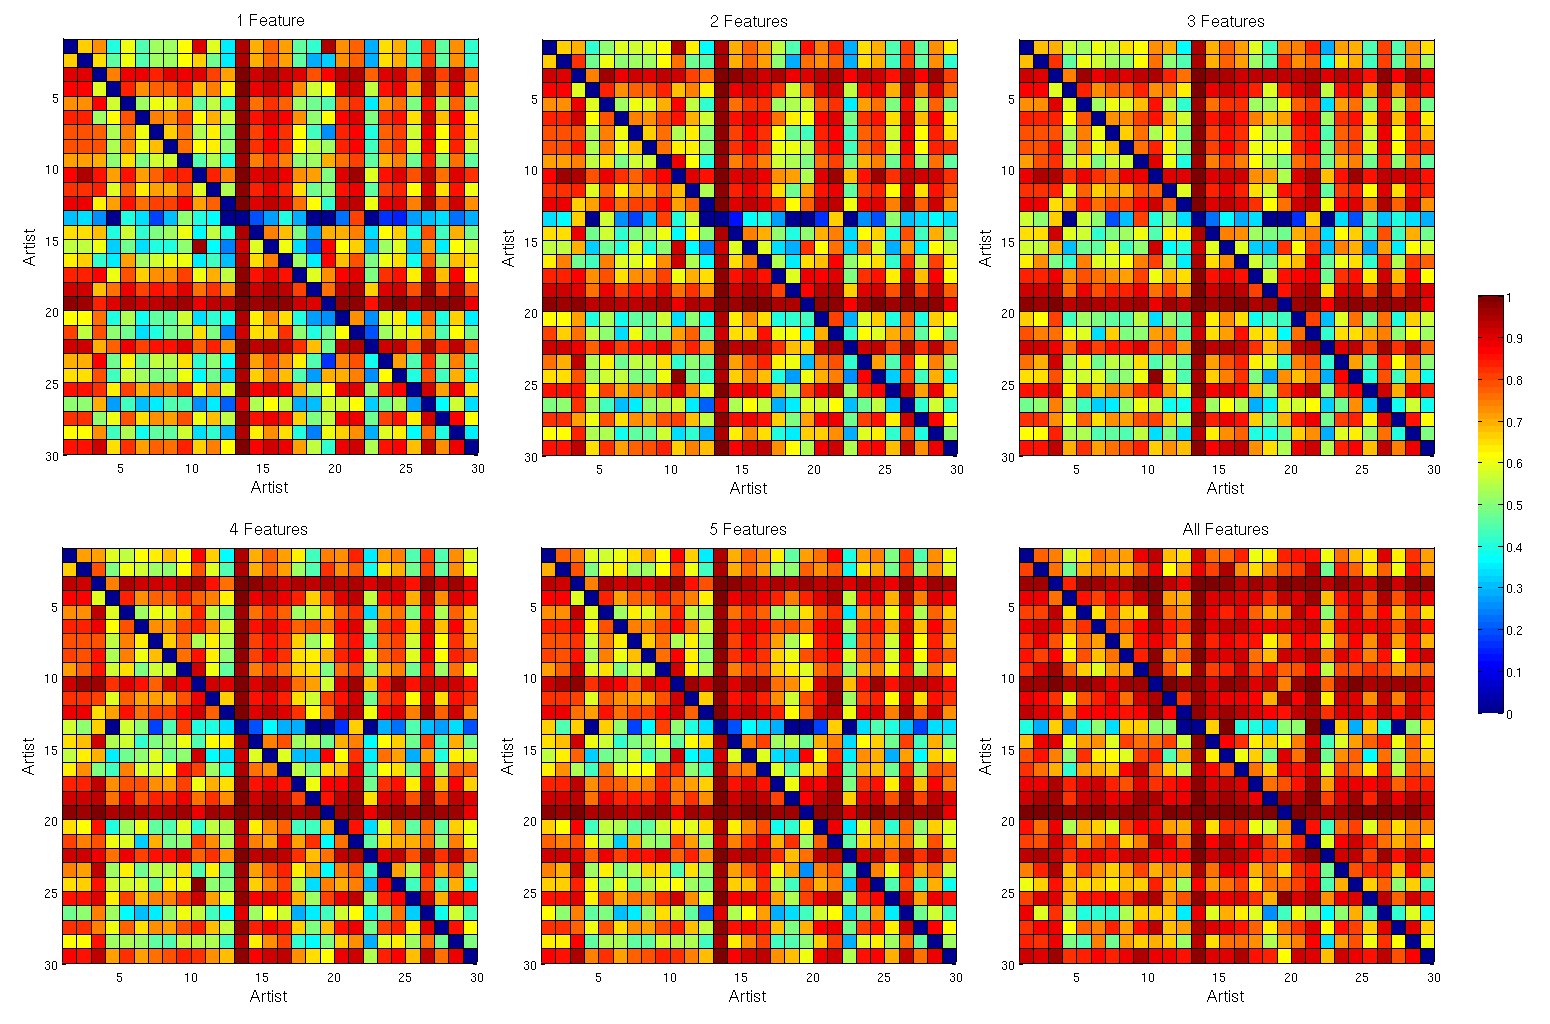
\includegraphics[width=1\linewidth]{img/experiment2results.png}
  \caption{The results of experiment 2 using different lengths of feature combinations. From left to right: 1-5 features and the last one is the result using all features.}
  \label{fig:experiment2results}
\end{figure*}

Figure \ref{fig:experiment2results} shows the results for this experiment using the linear SVM which was chosen in a greedy fashion based on the results found in table \ref{ex2optimizeresults}.
From left to right the figure shows the results of using: \textit{1} feature, \textit{2} features, \textit{3} features, \textit{4} features, \textit{5} features and \textit{all} features as the feature combination that is used by the classifier to classify images.
The results are plotted using an intensity mapping where each square represents the $F_1$-measure performance of separating the \textit{x} and \textit{y} artist.

The first thing that is noticable is that the intensity mappings are not symmetric.
This is because the $F_1$-measure was used here to evaluate the performance.
The measure is calculated by looking at the precision and recall of the positive class, so when the classes are turned around the $F_1$-measure will also turn into a different value.
Therefore in order to determine if two artists are separable, there is a need to look at the $F_1$-measure for both artists.
This is because for some artist pairs the $F_1$-measure of one artist has a value of 1 while the other has a value of 0.
This means that for those artist pairs the classifier has classified all images to one artist, which most of the time is caused by the non-uniform dataset.

Furthermore the figure shows that artists can be better separated by using more features.
The intensity mapping using all features shows that it has the highest overall $F_1$-measure.
However the more interesting mappings are the ones where only the top 1,2,3,4,5 features were used for classification.
Eventhough their performance is lower than using all the features it gives information about the most defining features that is used to separate an artist from another artist.

The intensity mappings using 1 to 5 features contains artists that have an overall high $F_1$-measure which shows that some artists can be separated from all other artists using only a few features.

\begin{table}[htb]
    \centering
    \begin{tabular}
        { | l | c |} 
        \hline
        Feature & Counts \\
        \hline
        gridEdgeRatio\_5 & 9 \\ 
        intEntropy & 4 \\ 
        edgeRatio & 4 \\ 
        avgRCells\_9 & 4 \\ 
        medIntCells\_2 & 3 \\
        medIntCells\_7 & 3 \\
        \hline 
    \end{tabular}
    \caption{Counts of features that were used to separate \textit{Kitsunebaka91} from the other artists.}
    \label{kitsune}
\end{table}

Table \ref{kitsune} shows the top 6 feature counts of features that were used to distinct \textit{Kitsunebaka91} from the other artists.
The features were counted whenever the $F_1$-measure of \textit{Kitsunebaka91} had an $F_1$-measure higher than 0.9, which indicates that the artist is separable from the other artist.
So the table details the reason why \textit{Kitsunebaka91} was separable.
The artwork of \textit{Kitsunebaka91} consists mostly of images where there is a white background with a drawing in the center of it.
This corresponds to the features found using this toolkit because table \ref{kitsune} shows that the edgeratio and intensity of the images are the dominant features to separate this artist from other artists.
Also the table shows that the \textit{GridEdgeRatio\_5} feature is used multiple times to separate this artist.
This again corresponds to the artist style because the \textit{GridEdgeRatio\_5} is the edgeratio value of the center cell of an image, the cell where the drawing of the artist lies.

Eventhough \textit{Kitsunebaka91} was seperable from most other artists, pairing \textit{Kitsunebaka91} with the artist \textit{Knuxtiger4} resulted in a lower $F_1$-measure of 0.7397 wheras the mean of all the scores was 0.91.
Inspecting the images of \textit{Knuxtiger4} showed that the artist mostly contained images that were drawings on a white background similar to that of \textit{Kitsunebaka91}.
Therefore it is not surprising that the score for that pair was lower than the average because the classifier could not seperate those images.
These results indicates that these results can be used to create a recommender system.

\subsection{Network experiments}
The network experiments have multiple goals, to analyse the dA network to establish global characteristics of the network, but also to find interesting sub-networks of artists and artworks which are of particular interest to investigate.

The dA network consists of 13 million registered users, doing a full analysis of the the whole network was impossible within the scope of the project. Therefore a network of the dA watchers functionality\footnote{a watcher is someone who indicates he likes an artist and would like to receive updates when that artist produces new artwork.} was extracted for all but casual artists, these latter can be destiguished with a $~$, indicating that they do not have a paid membership. This network formed the basis of our network experiments.

From this large network of professional artists three core-networks were extracted using the corefind algorithm, described in Algorithm \ref{alg:findcore}. The three cores correspond to three types of the $degree(j)$ function in that algorithm, namely - in-degree, out-degree and in+out-degree -. This has resulted in a core of artists that are "power-watchers" a core with "popular-watched" artists, and a last a mix of both.

%\begin{table}[htb]
%    \centering
 %   \begin{tabular}
  %      { | l | c | c | c | c | c | c|} 
 %       \hline
 %       Network & no. nodes & no. links & avg. node degree & corefind degree $x$ & $L_G$ & $L_{random}$ & $C_G$ & $C_{random}$ \\
%        \hline
%	prof. artists & 103'663 & 4'483'023 & 43.25 & & & & & \\
%         watchers-core & 1'701 & 139'285 & 81.88 & 43 & 2.15 & 1.69 & 0.20 & 0.048\\
%	watched-core & 1471 & 127'837 & 86.90 & 44 & 2.27 &  1.63 & 0.22 & 0.059\\
%	mixed-core & 1099 & 166'244 & 151.27 & 185 & 2.14  & 1.40 & 0.20 & 0.140 \\
 %   \end{tabular}
 %   \caption{Network statistics}
 %   \label{netstatistics}
%\end{table}
\subsubsection{results}
The results of the network experiments are presented in table \ref{tab:netstatistics}, as well as figure \ref{fig:results_core}.  For all networks statistics were extracted, unfortunately for the large professional users network statistics such as the characteristic path length were not possible to compute within the given time period.

\begin{table}[htb]
    \centering
    \begin{tabular}
        { | l | c | c | c | c | c | c|} 
        \hline
        Network &  prof.  & watchers & watched & mixed\\
	            &  artists & core & core & core \\
        \hline
	no. nodes $(n)$& 103'663 & 1'701 & 1471 & 1099 \\
	no. links & 4'483'023 & 139'285 & 127'837  & 166'244 \\
	avg. degree $(k)$& 43.25 & 81.88 & 86.90 & 151.27 \\
	corefind $\max x$ & & 43 & 44 & 185\\
	$L_G$ & & 2.15 & 2.27 & 2.14 \\
	$L_{random}$ & & 1.69 & 1.63 & 1.40 \\
	$C_G$ & & 0.20 & 0.22 & 0.20 \\
	$C_{random}$ & & 0.048 & 0.059 & 0.140 \\
	\hline
    \end{tabular}
    \caption{Network statistics}
    \label{tab:netstatistics}
\end{table}


\begin{figure}[htb]
  \centering
  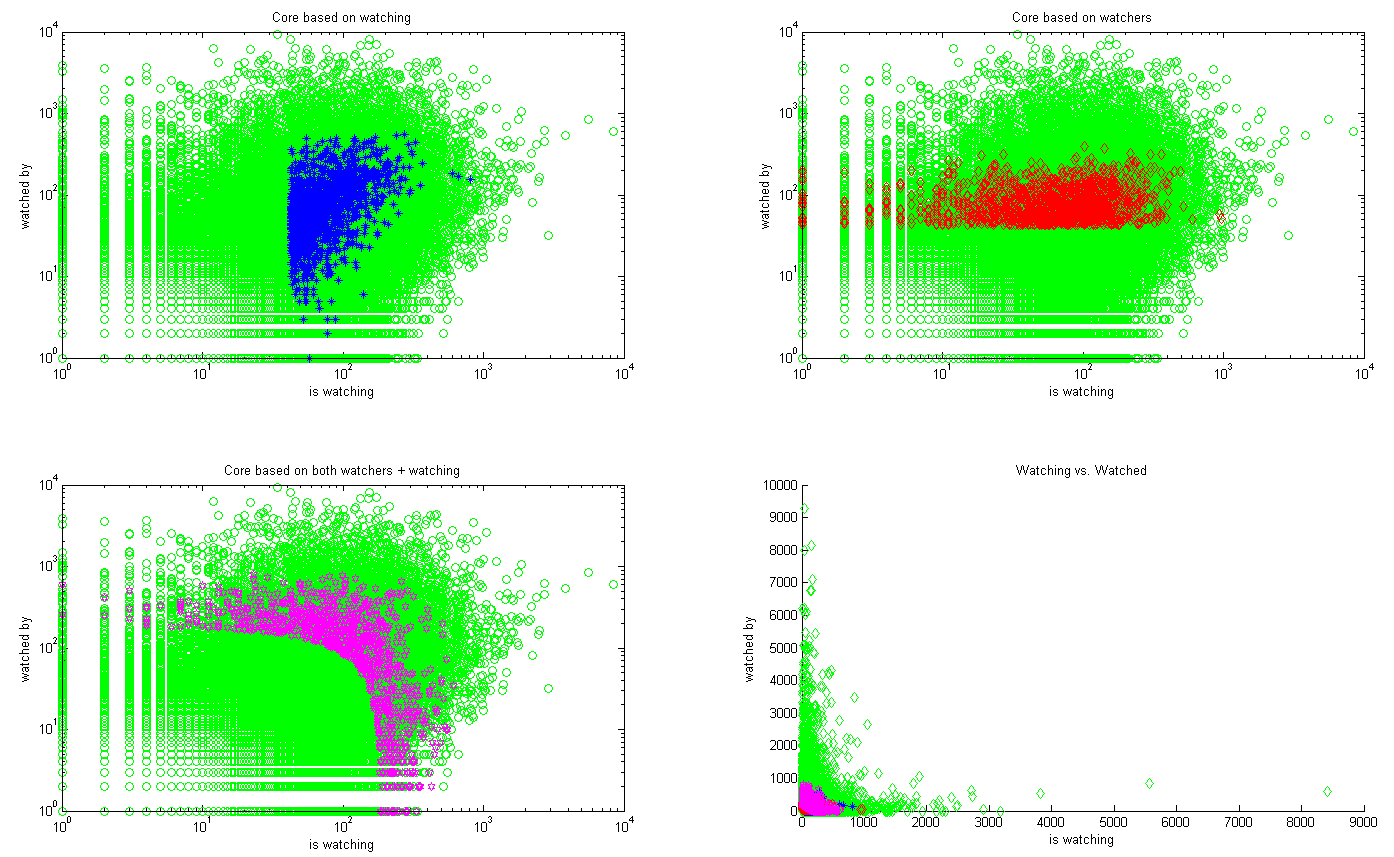
\includegraphics[width=1\linewidth]{img/core.png}
  \caption{Core networks, the degree of watching versus being watched.  The green dots represent the whole professional network, while the blue represends the watchers-core, red the watched and pink the mixed core, the last subfigure shows the power-law behavior of the degree distributions.}
  \label{fig:results_core}
\end{figure}
\subsubsection{discussion}
As described in section \ref{proposed}.\ref{proposed_networks}, a network can be considered small-world when $L_G\approx L_{random}$ and $C_G \gg C_{random}$. All core networks have a clustering coefficient larger than a comparable random network, though the mixed core is close to the random network. The characteristic path lengths are longer than their random network equivalents. This is most likely due to the relatively small size of the networks, the paths are still significantly smaller than $L_{lattice}=\frac{n}{2k}$. We therefore conclude that the core's of dA can be considered small-world networks.  
